%--------------------------------------------
% PACKAGES AND OTHER DOCUMENT CONFIGURATIONS
%--------------------------------------------

\documentclass{scrartcl}

\reversemarginpar % Move the margin to the left of the page 

\usepackage[dvipsnames]{xcolor}
\definecolor{carmine}{rgb}{0.59, 0.0, 0.09}
\definecolor{deepchestnut}{rgb}{0.73, 0.31, 0.28}

\newcommand{\MarginText}[1]{\marginpar{\raggedleft\itshape\small#1}} % New command defining the margin text style

\usepackage[nochapters]{classicthesis} % Use the classicthesis style for the style of the document
\usepackage[LabelsAligned]{currvita} 	% Use the currvita style for the layout of the document
\usepackage{geometry}
 \geometry{
 a4paper,
 total={170mm,257mm},
 left=17mm,
 right=17mm,
 top=20mm,
 }
\usepackage{wrapfig}
\usepackage{graphicx}
\usepackage{enumitem}
\usepackage{hyperref} % Required for adding links and customizing them
\hypersetup{colorlinks, breaklinks, urlcolor=deepchestnut, linkcolor=blue} % Set link colors

\usepackage{scrextend}

\renewcommand{\cvheadingfont}{\LARGE\color{Maroon}} % Font color of your name at the top

\newlength{\datebox}\settowidth{\datebox}{Sep 2019 - Feb 2020} % Set the width of the date box in each block

\newcommand{\NewEntry}[3]{\noindent\hangindent=1em\hangafter=0 \parbox{\datebox}{\small \textit{#1}}\hspace{1.5em} #2 #3
  \vspace{0.5em}
}
  
\newcommand{\NewItemEntry}[2]{
  \noindent
  \begin{tabular}[r]{p{2.5cm} p{14.0cm}}
    \-\hspace{0.5cm} \small \textit{#1}
    &
    \begin{itemize}
      \vspace{-0.65cm}
      \item[$\cdot$] #2
    \end{itemize}
  \end{tabular}
  \vspace{-0.2cm}
}

\newcommand{\NewLanguageEntry}[2]{
  \noindent
  \begin{tabular}[r]{p{3cm} p{13.5cm}}
    \-\hspace{0.5cm} \small \textsc{#1}
    &
    \begin{itemize}
      \vspace{-0.65cm}
      \item #2
    \end{itemize}
  \end{tabular}
  \vspace{-0.2cm}
}





%------------------------------------------
%          CONTACT INFORMATION
%------------------------------------------

\vspace{0.5em}

\newcommand{\rdate}[1]{\textsc{#1}}

\begin{document}

\hfill \rdate{\today}

\begin{cv}{\spacedallcaps{Alberto Dinelli}}
  \small
  
\vspace{2.0em} % Your name

%\begin{wrapfigure}{r}{3.7cm} % r indica la posizione (right) e 3.5cm indica lo spazio che prende
%  \centering
%  \vspace{-20pt} % crea uno spazio negativo che porta in su la foto
  %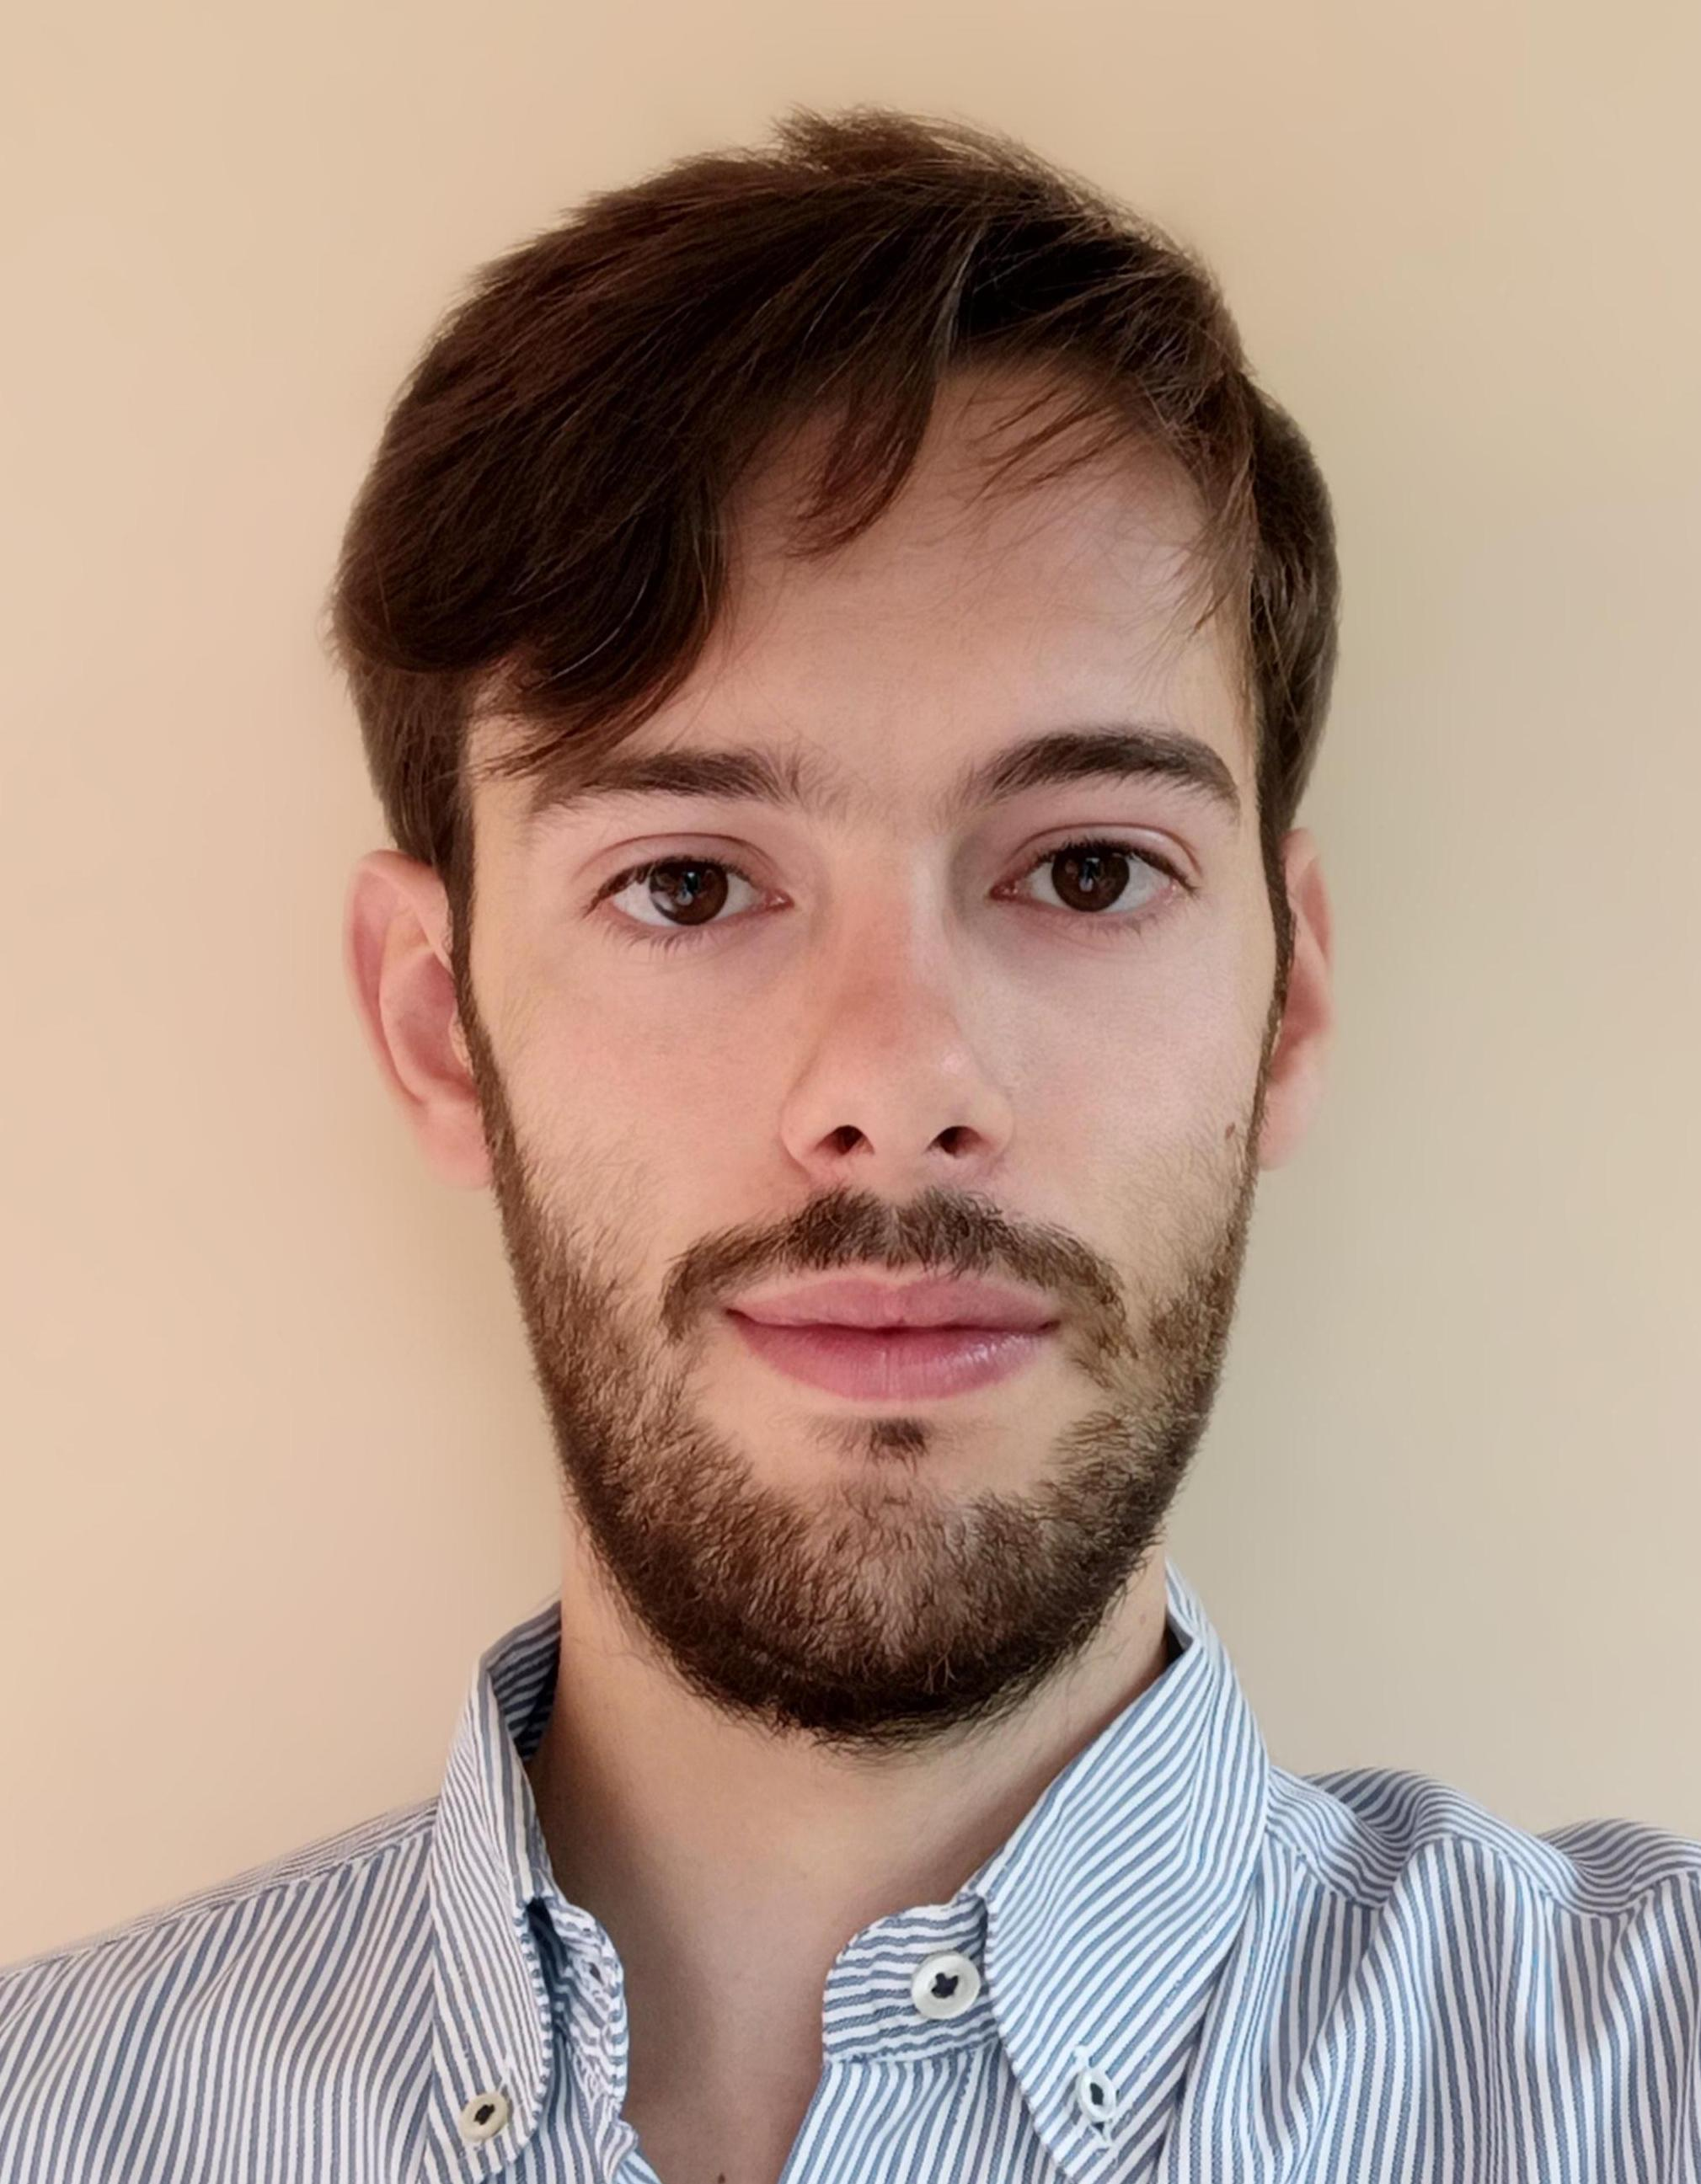
\includegraphics[width=3.7cm]{Photo_ID_Fr}
%%  \vspace{25pt} % crea uno spazio positivo per compensare
%\end{wrapfigure}

\NewEntry{Born in}{Lucca (Italia),}{07/10/1997} % Birthplace and date

\NewEntry{email}{\href{mailto:alberto.dinelli@u-paris.fr}{alberto.dinelli@u-paris.fr}} % Email address

\NewEntry{address}{Laboratoire Matière et Systèmes Complexes \\\-\hspace{4.0cm}UMR 7057 $\cdotp$ Université de Paris\\
  \-\hspace{4.0cm}10 rue Alice Domon et Léonie Duquet\\
  \-\hspace{4.0cm}75205 Paris CEDEX 13 (\textit{France})}

\NewEntry{website}{\href{https://adinelli.github.io/}{adinelli.github.io}}

\vspace{1em}

\par\noindent\rule{\textwidth}{0.4pt}

\vspace{1.5em}











%------------------------
%	EDUCATION
%------------------------

\noindent\spacedallcaps{\textbf{Education}}\vspace{1em}
\small

\begin{tabular}{p{4cm}|p{14cm}} % <=============================
  
  \begin{tabular}[t]{@{}l@{}}\parbox{\datebox}{Sept 2024 - Present}
  \end{tabular}
  & \large{\textcolor{carmine}{\textbf{Postdoc}}}
  \newline
  \normalsize\texttt{Biochemistry department}  $\cdotp$ \textit{University of Geneva}\\[0.2cm]
        %\\ & in collaboration with \texttt{Massachussets Institute of Technology} $\cdotp$ \textit{Boston}\\[0.2cm]%
	\begin{tabular}{p{4.5cm} p{13.5cm}}
	& \footnotesize\textbf{Advisor:} Karsten Kruse.
	\end{tabular}\\
  \multicolumn{2}{c}{}\\[0.5cm]
  
  \begin{tabular}[t]{@{}l@{}}\parbox{\datebox}{Oct 2021 - Aug 2024}
  \end{tabular}
  & \large{\textcolor{carmine}{\textbf{Ph.D. - Physique en Île de France}}}
  \newline
  \normalsize\texttt{Laboratoire Matière et Systèmes Complexes, Université Paris Cité}  $\cdotp$ \textit{Paris}\\[0.2cm]
        %\\ & in collaboration with \texttt{Massachussets Institute of Technology} $\cdotp$ \textit{Boston}\\[0.2cm]%
	\begin{tabular}{p{4.5cm} p{13.5cm}}
	& \footnotesize\textbf{Subject:} Scalar Active Matter across scales.\\
	& \footnotesize\textbf{Supervisor:} Julien Tailleur.
	\end{tabular}\\[0.5cm]
  \begin{tabular}[t]{@{}l@{}}\parbox{\datebox}{\small Oct 2023 - Nov 2023}
  \end{tabular}
  & \small{$\>\>\cdotp\>\>$} \small{Visiting period at MIT, group of Prof. J. Tailleur $\cdotp$ \textit{Cambridge}, US}\\[0.1cm]
  \begin{tabular}[t]{@{}l@{}}\parbox{\datebox}{\small Jul 2023}
  \end{tabular}
  & \small{$\>\>\cdotp\>\>$} \small{Visiting period at YITP, group of Prof. H. Hayakawa $\cdotp$ \textit{Kyoto}, JP}\\[0.1cm]
  \begin{tabular}[t]{@{}l@{}}\parbox{\datebox}{\small Oct 2022}
  \end{tabular}
  & \small{$\>\>\cdotp\>\>$} \small{Visiting period at MIT, group of Prof. J. Tailleur $\cdotp$ \textit{Cambridge}, US}\\
  \multicolumn{2}{c}{}\\[0.5cm]
  
  \begin{tabular}[t]{@{}l@{}}\parbox{\datebox}{Sep 2019 - Jul 2021}
  \end{tabular}
  & \large{\textcolor{carmine}{\textbf{Master in Physics of Complex Systems (\href{http://www.pcs.polito.it/educational_tracks/international_track}{International Track})}}}\\
  & \normalsize\texttt{Politecnico di Torino}  $\cdotp$ \textit{Torino}\\
  & \texttt{Université Paris-Saclay}, \texttt{Sorbonne Université}, \texttt{Université de Paris} $\>\>\cdotp$ \textit{Paris}\\
  & \texttt{SISSA}, \texttt{ICTP} $\cdotp$ \textit{Trieste}\\[0.2cm]
  \begin{tabular}{p{4.5cm} p{13.5cm}}
	& \footnotesize\textbf{Italian degree mark:} 110/110 cum laude\\
	& \footnotesize\textbf{French M2 mark:} 18/20\\
	& \footnotesize\textbf{Thesis:} Self-organization of active mixtures.\ $\cdotp$ \textbf{Supervisor:} Julien Tailleur.
	\end{tabular}\\
  \multicolumn{2}{c}{} \\[0.5cm]
  
  \begin{tabular}[t]{@{}l@{}}\parbox{\datebox}{Sep 2016 - Jul 2019}
  \end{tabular}
  & \large{\textcolor{carmine}{\textbf{Bachelor degree in Physics}}}\\
  & \normalsize\texttt{Università di Pisa}  $\cdotp$ \textit{Pisa}\\[0.2cm]
  \begin{tabular}{p{4.5cm} p{13.5cm}}
	& \footnotesize\textbf{Degree mark:} 110/110 cum laude\\
	& \footnotesize\textbf{Thesis:} Rayleigh Taylor instability on a thin layer of fluid accelerated by the \\[-0.1cm] 
	& \footnotesize radiation pressure.\  $\cdotp$ \textbf{Supervisor:} Francesco Pegoraro.
  \end{tabular}\\
  
  \if{
  \multicolumn{2}{c}{} \\[0.5cm]
  \begin{tabular}[t]{@{}l@{}}\parbox{\datebox}{2011 - 2016}
  \end{tabular}
  & \large{\textcolor{carmine}{\textbf{Scientific high school diploma}}}\\
  & \normalsize\texttt{Liceo Scientifico A. Vallisneri}  $\cdotp$ \textit{Lucca}\\[0.2cm]
  \begin{tabular}{p{4.5cm} p{13.5cm}}
	& \footnotesize\textbf{Degree mark:} 100/100 cum laude\\
	\end{tabular}\\
  }\fi
  
\end{tabular}
\vspace{1em}

\par\noindent\rule{\textwidth}{0.4pt}

\vspace{1.5em}









%-----------------------------
%	   TEACHING
%-----------------------------

\noindent\spacedallcaps{\textbf{Teaching}}\vspace{1em}
\def\v{-0.1cm}

\NewItemEntry{2021 - 2024}{Teaching assistant, \textit{Physics of Materials} (Bachelor, 1st year) $\cdotp$ IUT Pajol (\textit{Paris})}\\[\v]
\NewItemEntry{}{Teaching assistant, \textit{Photonics} (Bachelor, 2nd year) $\cdotp$ IUT Pajol (\textit{Paris})}

\vspace{1em}

\par\noindent\rule{\textwidth}{0.4pt}

\vspace{1.5em}


\newpage

%---------------------------------
%	PUBLICATIONS
%---------------------------------

\noindent\spacedallcaps{\textbf{Publications}}\vspace{1em}
\small
\begin{enumerate}
\item \underline{A. Dinelli}, J. O’Byrne and J. Tailleur, ``Fluctuating hydrodynamics of active particles interacting via chemotaxis and quorum sensing: static and dynamics''. \href{https://arxiv.org/abs/2402.05072}{arXiv:2402.05072} (2024).
\item \underline{A. Dinelli}, J. O’Byrne, A. Curatolo, Y. Zhao, P. Sollich, J. Tailleur, ``Non-reciprocity across scales in active mixtures''. \href{https://doi.org/10.1038/s41467-023-42713-5}{Nature Communications} 14, 7035 (2023). 
\end{enumerate}
  

\par\noindent\rule{\textwidth}{0.4pt}

\vspace{1.5em}






%---------------------------------
%	TALKS
%---------------------------------

\noindent\spacedallcaps{\textbf{Talks}}\vspace{1em}

\def\v{-0.1cm}

\small
\NewItemEntry{2024-04}{Seminar in K. Kruse's group, (Université de Genève, \textit{Geneva})}\\[\v]
\NewItemEntry{2024-02}{Seminar at \textit{\href{https://indico.ictp.it/event/10459/session/58/contribution/56}{Spring College of Physics of Complex Systems 2024}} (ICTP, \textit{Trieste})}\\[\v]
\NewItemEntry{2024-01}{Flash talk at \textit{\href{https://jstat.phys.ens.fr/fr}{Journées de Physique Statistique 2024}} (ENS, \textit{Paris})}\\[\v]
\NewItemEntry{2024-01}{Seminar in M. Shelley's group, (CCB, Flatiron Institute, \textit{New York})}\\[\v]
\NewItemEntry{2023-10}{Seminar in D. Nelson's group, (Harvard University, \textit{Cambridge})}\\[\v]
\NewItemEntry{2023-10}{Seminar in P. Mehta and K. Koroloev's groups, (Boston University, \textit{Boston})}\\[\v]
\NewItemEntry{2023-10}{Seminar in M. Hagan's group, (Brandeis University, \textit{Waltham})}\\[\v]
\NewItemEntry{2023-08}{Contributed talk at \textit{\href{https://confit.atlas.jp/guide/event/statphys28/subject/T6-11C-02/detail}{STATPHYS28}}, (University of Tokyo, \textit{Tokyo})}\\[\v]
\NewItemEntry{2023-08}{Contributed talk at \textit{\href{https://www2.yukawa.kyoto-u.ac.jp/~noneq-active-matter2023/index.php}{Frontiers in nonequilibrium physics: Active matter, topology and beyond}}, (YITP, \textit{Kyoto})}\\[\v]
\NewItemEntry{2023-07}{\textit{\href{https://www2.yukawa.kyoto-u.ac.jp/~non-equilibrium/seminar.html}{Seminar}} at YITP, Advanced Statistical Dynamics Group, (YITP, \textit{Kyoto})}\\[\v]
\NewItemEntry{2023-06}{Contributed talk at  \textit{\href{https://www.edpif.org/journee/2023/index_en.html}{EDPIF Scientific Day}}, (Sorbonne University, \textit{Paris})}\\[\v]
\NewItemEntry{2023-03}{Seminar at Institut Curie, Theory Group (Institut Curie, \textit{Paris})}\\[\v]
\NewItemEntry{2023-01}{Flash talk at \textit{\href{https://jstat.phys.ens.fr/fr}{Journées de Physique Statistique 2023}} (ENS, \textit{Paris})}\\[\v]
\NewItemEntry{2022-11}{Contributed talk at \textit{\href{https://etn-phymot.eu/phymot-workshop/}{Physics of Microbial Motility Workshop}} (ESPCI, \textit{Paris})}\\[\v]
\NewItemEntry{2022-10}{Talk at \textit{\href{https://sites.google.com/umass.edu/gbasm2022/home}{Greater Boston Area Statistical Mechanics Meeting}} \if{[replacing Prof. Julien Tailleur]}\fi (UMass-Amherst, \textit{Amherst})} \\[\v]
\NewItemEntry{2022-10}{Seminar at MIT Physics of Living Systems (MIT, \textit{Cambridge})}\\[\v]
\NewItemEntry{2022-06}{Contributed talk at the CECAM Workshop: \textit{\href{https://www.cecam.org/workshop-details/1111}{New Fronteers in Liquid Matter}} (Sorbonne Jussieu, \textit{Paris})}\\[\v]
\NewItemEntry{2022-01}{Flash talk at \textit{\href{https://jstat.phys.ens.fr/fr}{Journées de Physique Statistique 2022}} (ENS, \textit{Paris})}\\[\v]
\NewItemEntry{2021-11}{Flash talk at \textit{\href{https://training.institut-curie.org/courses/multiscale-integration-in-biological-systems-3}{Multiscale integration in Biological Systems}} (Insitut Curie, \textit{Paris})}
  
  


\vspace{1em}

\par\noindent\rule{\textwidth}{0.4pt}

\vspace{1.5em}


%---------------------------------
%	POSTERS
%---------------------------------

\noindent\spacedallcaps{\textbf{Poster presentations}}\vspace{1em}

\NewItemEntry{2023-08}{\textit{\href{https://www2.yukawa.kyoto-u.ac.jp/~yitp-ysf2022/index.php}{Perspectives on Non-Equilibrium Statistical Mechanics}} (YITP, \textit{Tokyo})}\\[\v]
\NewItemEntry{2023-06}{\textit{\href{https://www.pks.mpg.de/amsce23}{Active matter at surfaces and in complex environments}} (MPIPKS, \textit{Dresden})}\\[\v]
\NewItemEntry{2023-05}{\textit{\href{https://indico.ictp.it/event/10169/}{Workshop on Signatures of Nonequilibrium fluctuations in life}} (ICTP, \textit{Trieste})}\\[\v]
\NewItemEntry{2022-12}{\textit{\href{https://everevol.sciencesconf.org/}{Population dynamics: from rare events to evolution}} (Université Grenoble Alpes, \textit{Grenoble})}


\vspace{1em}

\par\noindent\rule{\textwidth}{0.4pt}

\vspace{1.5em}



\newpage

%--------------------------------
%	COMPUTER SKILLS
%--------------------------------

\noindent\spacedallcaps{\textbf{Computer Skills}}
\vspace{1em}
\small

\NewItemEntry{Intermediate}{Julia, \textsc{Matlab}, \textsc{Mathematica}}\\[\v]
\NewItemEntry{Advanced}{Python, C, awk, bash, \LaTeX}

\vspace{1.0em} % Extra space between major sections

\par\noindent\rule{\textwidth}{0.4pt}

\vspace{1.5em}















%----------------------------------------
%	OTHER INFORMATION
%----------------------------------------

\noindent\spacedallcaps{\textbf{Other Information}}
\vspace{1em}


\textcolor{carmine}{\textbf{Awards}}
\vspace{1em}

\small

\NewItemEntry{2023}{International Mobility Fellowship \href{https://www.edite-de-paris.fr/universite-paris-cite-bdmi/}{BDMI}}\\[\v]
\NewItemEntry{2021 - 2024}{IdEX International PhD Fellowship (\href{https://www.mastere.tn/en/university-of-paris-doctoral-fellowship-program-2021/}{Link})}\\[\v]
\NewItemEntry{2020 - 2021}{Paris-Saclay International Master's Scolarship (\href{https://www.universite-paris-saclay.fr/en/admission/bourses-et-aides-financieres/international-masters-scholarships-program}{Link})}


%------------------------------------------------

\vspace{1em}



\if{
\textcolor{carmine}{\textbf{Achievements}}
\vspace{1em}

\small

\NewItemEntry{Feb 2021}{1$^{st}$ position in the French ranking of the Physics of Complex Systems master}\\
\NewItemEntry{Jun 2019}{1$^{st}$ position in the admission test to Physics of Complex Systems master}
%\NewItemEntry{Apr 2016}{Participation to the Italian national phase of \href{https://www.olifis.it/index.php/informazioni/30-anni}{Physics Olympiad for high schools}}
}\fi

%------------------------------------------------

\vspace{1em}

\normalsize

\if{
\textcolor{carmine}{\textbf{Attendance to conferences}}
\vspace{1em}
\small

\NewItemEntry{Aug 2023}{\textit{\href{https://statphys28.org/}{STATPHYS28}} (University of Tokyo, \textit{Tokyo})}\\
\NewItemEntry{Jul 2023}{\textit{\href{https://www2.yukawa.kyoto-u.ac.jp/~yitp-ysf2022/index.php}{Perspectives on Non-Equilibrium Statistical Mechanics}} (YITP, \textit{Kyoto})}\\
\NewItemEntry{Jul 2023}{\textit{\href{https://www2.yukawa.kyoto-u.ac.jp/~noneq-active-matter2023/index.php}{Frontiers in nonequilibrium physics: Active matter, topology and beyond}} (YITP, \textit{Kyoto})}\\
\NewItemEntry{Jun 2023}{\textit{\href{https://www.pks.mpg.de/amsce23}{Active matter at surfaces and in complex environments}} (MPIPKS, \textit{Dresden})}\\
\NewItemEntry{May 2023}{\textit{\href{https://indico.ictp.it/event/10169/}{Workshop on Signatures of Nonequilibrium fluctuations in life}} (ICTP, \textit{Trieste})}\\
\NewItemEntry{Jan 2023}{\textit{\href{https://jstat.phys.ens.fr/fr}{Journées de Physique Statistique 2023}} (ENS, \textit{Paris})}\\
\NewItemEntry{Dec 2022}{\textit{\href{https://everevol.sciencesconf.org/}{Population dynamics: from rare events to evolution}} (Université Grenoble Alpes, \textit{Grenoble})}\\
\NewItemEntry{Nov 2022}{\textit{\href{https://etn-phymot.eu/phymot-workshop/}{Physics of Microbial Motility Workshop}} (ESPCI, \textit{Paris})}\\
\NewItemEntry{Oct 2022}{\textit{\href{https://sites.google.com/umass.edu/gbasm2022/home}{Greater Boston Area Statistical Mechanics Meeting}} (UMass-Amherst, \textit{Amherst})}\\
\NewItemEntry{Aug 2022}{\textit{\href{https://www.lorentzcenter.nl/active-matter-the-next-25-years-2022.html}{Active Matter: The Next 25 Years 2022}} (Lorentz Center, \textit{Leiden})}\\
\NewItemEntry{Jul 2022}{CECAM Workshop: \href{https://www.cecam.org/workshop-details/1111}{\textit{New Fronteers in Liquid Matter}} (Sorbonne Jussieu, \textit{Paris})}\\
\NewItemEntry{Jun 2022}{Summer school on \textit{\href{https://www.institut-pascal.universite-paris-saclay.fr/en/scientific-programs/disorder-complex-systems}{Disorder in Complex Systems}} (Institut Pascal, \textit{Orsay})}\\
\NewItemEntry{Jan 2022}{\textit{\href{https://jstat.phys.ens.fr/fr}{Journées de Physique Statistique 2022}} (ENS, \textit{Paris})}\\
\NewItemEntry{Nov 2021}{\textit{\href{https://training.institut-curie.org/courses/multiscale-integration-in-biological-systems-3}{Multiscale integration in Biological Systems}} (Institut Curie, \textit{Paris})}\\
\NewItemEntry{Jun 2021}{\textit{\href{https://www.ipht.fr/Meetings/BegRohu2021/index.html}{Beg Rohu Summer School}} on Statistical Physics and Emergent Phenomena in Biology} \\
\NewItemEntry{Mar 2021}{\textit{\href{http://indico.ictp.it/event/9442/}{Spring College}} on the Physics of Complex Systems (ICTP, SISSA, \textit{Trieste})}\\
\NewItemEntry{Jan 2021}{\href{http://irs.math.cnrs.fr/2021/}{IRS 2021} Inhomogeneours Random Systems 2021}\\
\NewItemEntry{Aug 2019}{\href{https://www.iaps.info/icps/previous-icpss/icps-2019-in-germany/}{ICPS} International Conference of Physics Students (\textit{Köln})}\\
\NewItemEntry{Nov 2018}{\href{http://ai-sf.it/gipe18/}{GIPE} German-Italian Physics Exchange (\textit{Trieste})}\\
\NewItemEntry{Sep 2015}{University orientation course held by Scuola Normale Superiore di Pisa (\href{https://www.sns.it/it/orientamento}{Link}) (\textit{San Miniato})}

\vspace{1em}
}\fi

%------------------------------------------------

\normalsize

\textcolor{carmine}{\textbf{Languages}}
\vspace{1em}

\small
\NewItemEntry{Italian}{Mothertongue}\\[\v]
\NewItemEntry{English}{Advanced C2 (Cambridge Proficiency Certificate in 2015)}\\[\v]
\NewItemEntry{French}{Advanced}\\[\v]

\date{}
\end{cv}

\end{document}
